\documentclass[12pt]{article}
\usepackage[T1, T2A]{fontenc}
\usepackage[utf8]{inputenc}
\usepackage[russian]{babel}
\usepackage{hyperref}
\usepackage{graphicx}
\graphicspath{ {../Images/} }

\author{Григорий Матюхин}
\date{\today}
\title{Лабораторная работа \textnumero4.\\Работа с программными пакетами}

\begin{document}
\maketitle
\newpage
\tableofcontents
\newpage
\section{Цель работы}
Получить навыки работы с репозиториями и менеджерами пакетов.

\section{Последовательность выполнения работы}

\subsection{Работа с репозиториями}
\begin{enumerate}
	\item В консоли перейдите в режим работы суперпользователя.
	\item Перейдите в каталог \texttt{/etc/yum.repos.d} и изучите содержание каталога и файлов репозиториев:
	      \\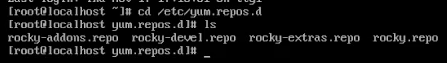
\includegraphics{1.png}
	\item Выведите на экран список репозиториев и поясните полученную информацию.
	      \\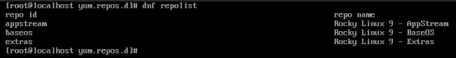
\includegraphics{2.png}
	\item Выведите на экран список пакетов, в названии или описании которых есть слово user и поясните полученную информацию.
	\item Установите \texttt{nmap}, предварительно изучив информацию по имеющимся пакетам. Поясните разницу между \texttt{dnf install nmap} и \texttt{dnf install nmap\*}.
	      \\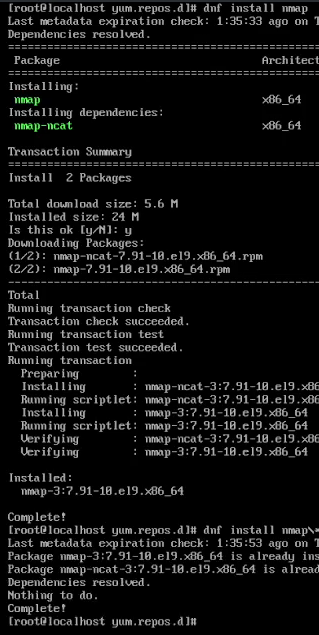
\includegraphics{3.png}
	\item Удалите \texttt{nmap}:
	      \\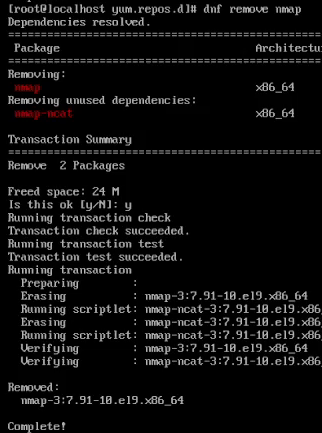
\includegraphics{4.png}
	\item Получите список имеющихся групп пакетов, затем установите группу пакетов \texttt{RPM Development Tools}:
	      \\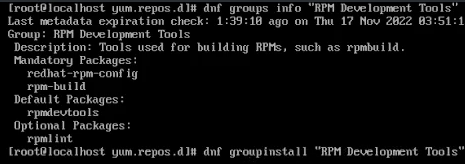
\includegraphics{5.png}
	\item Посмотрите историю использования команды \texttt{dnf} и отмените последнее, например шестое по счёту, действие:
	      \\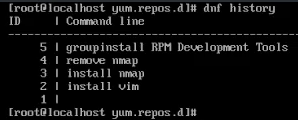
\includegraphics{6.png}

\end{enumerate}

\subsection{Использование rpm}
Предположим, что требуется установить текстовый браузер \texttt{lynx} из rpm-пакета
\begin{enumerate}
	\item Скачайте rpm-пакет \texttt{lynx}:
	\item Найдите каталог, в который был помещён пакет после загрузки:
	\item Перейдите в этот каталог и затем установите rpm-пакет:
	      \\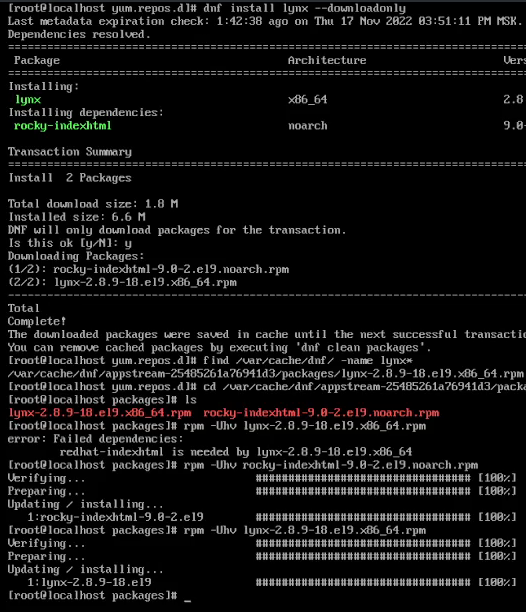
\includegraphics{7.png}
	\item Определите расположение исполняемого файла:
	\item Используя \texttt{rpm}, определите по имени файла, к какому пакету принадлежит \texttt{lynx} и получите дополнительную информацию о содержимом пакета:
	      \\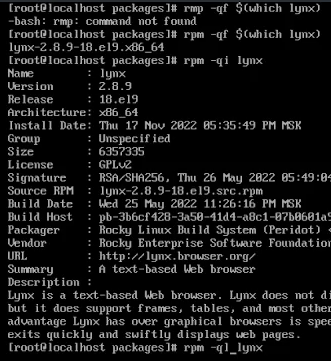
\includegraphics{8.png}
	\item Получите список всех файлов в пакете, используя, а также выведите перечень файлов с документацией пакета, посмотрите файлы документации, применив команду \texttt{man lynx}.
	      \\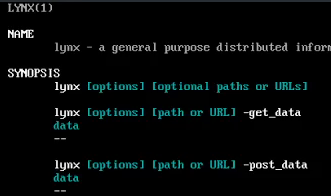
\includegraphics{9.png}
	\item Выведите на экран перечень и месторасположение конфигурационных файлов пакета:
	\item Выведите на экран расположение и содержание скриптов, выполняемых при установке пакета и поясните, для чего предназначены скрипты, если они есть.
	      \\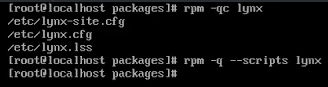
\includegraphics{10.png}
	\item В отдельном терминале под своей учётной записью запустите текстовый браузер \texttt{lynx}, чтобы проверить корректность установки пакета.
	      \\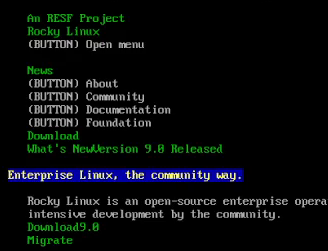
\includegraphics{11.png}
	\item Вернитесь в терминал с учётной записью \texttt{root} и удалите пакет:
	      \\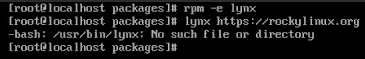
\includegraphics{12.png}
\end{enumerate}

Предположим, что требуется из rpm-пакетов установить \texttt{dnsmasq}\\ (DNS-, DHCP- и TFTP-сервер).
\begin{enumerate}
	\item Установите пакет \texttt{dnsmasq} и определите расположение исполняемого файла:
	\item Определите по имени файла, к какому пакету принадлежит \texttt{dnsmasq} и получите дополнительную информацию о содержимом пакета:
	\item Получите список всех файлов в пакете, а также выведите перечень файлов с документацией пакета, посмотрите файлы документации, применив команду \texttt{man dnsmasq}.
	      \\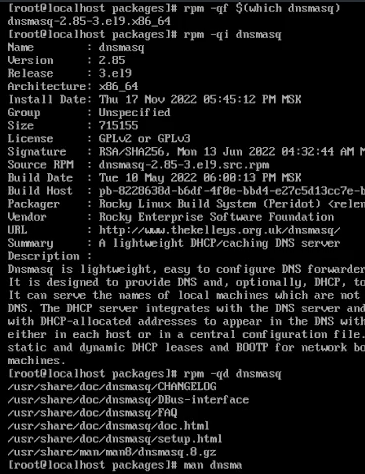
\includegraphics{13.png}
	\item Выведите на экран перечень и месторасположение конфигурационных файлов пакета:
	\item Выведите на экран расположение и содержание скриптов, выполняемых при установке пакета и поясните, для чего предназначены скрипты.
	      \\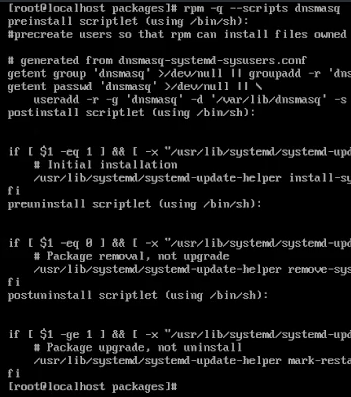
\includegraphics{14.png}
	\item Вернитесь в терминал с учётной записью \texttt{root} и удалите пакет:
	      \\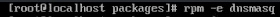
\includegraphics{15.png}
\end{enumerate}

\section{Контрольные вопросы}
\begin{enumerate}
	\item Какая команда позволяет вам искать пакет \texttt{rpm}, содержащий файл \texttt{useradd}?\\
	      \texttt{dnf provides <file-name>}
	\item Какие команды вам нужно использовать, чтобы показать имя группы \texttt{dnf}, которая содержит инструменты безопасности и показывает, что находится в этой группе?\\
	      \texttt{dnf groupinfo <group-name>}
	\item Какая команда позволяет вам установить rpm-пакет, который вы загрузили из Интернета и который не находится в репозиториях?\\
	      \texttt{dnf install <path-to-rpm>}
	\item Вы хотите убедиться, что пакет rpm, который вы загрузили, не содержит никакого опасного кода сценария. Какая команда позволяет это сделать?\\
	      Если мы доверяем создателю пакета, но не самому пакету, который мы скачали не из репозитория, то, используя плагин \texttt{dnf-plugin-verify} мы можем проверить контрольную сумму пакета используя \texttt{dnf verify-all}.
	\item Какая команда показывает всю документацию в rpm?\\
	      \texttt{rpm -qd <programm-name>}
	\item Какая команда показывает, какому пакету rpm принадлежит файл?\\
	      \texttt{dnf provides <file-name>}
\end{enumerate}

\section{Вывод}
В ходе выполнения данной работы я получил навыки работы с репозиториями и менеджерами пакетов.

\end{document}
